\documentclass[11pt,a4paper]{ctexart}
% Shared preamble for the assignment reports. Use with:
%   \documentclass[11pt,a4paper]{ctexart}  (XeLaTeX)
%   % Shared preamble for the assignment reports. Use with:
%   \documentclass[11pt,a4paper]{ctexart}  (XeLaTeX)
%   % Shared preamble for the assignment reports. Use with:
%   \documentclass[11pt,a4paper]{ctexart}  (XeLaTeX)
%   \input{../common/preamble.tex}
\usepackage[margin=2.3cm]{geometry}
\setmainfont{texgyretermes}[Extension=.otf,UprightFont=*-regular,BoldFont=*-bold,ItalicFont=*-italic,BoldItalicFont=*-bolditalic]
\setsansfont{texgyreheros}[Extension=.otf,UprightFont=*-regular,BoldFont=*-bold,ItalicFont=*-italic,BoldItalicFont=*-bolditalic]
\setmonofont{texgyrecursor}[Extension=.otf,UprightFont=*-regular,BoldFont=*-bold,ItalicFont=*-italic,BoldItalicFont=*-bolditalic]
\usepackage{amsmath,amssymb,mathtools,bm}
\usepackage{graphicx}
\usepackage{booktabs,multirow,makecell,array,tabularx}
\usepackage[table]{xcolor}
\usepackage[most]{tcolorbox}
\usepackage{enumitem}
\usepackage{listings}
\usepackage{subcaption}
\usepackage{siunitx}
\usepackage[hidelinks]{hyperref}
\usepackage[nameinlink,noabbrev]{cleveref}
\usepackage{float}

\setlength{\emergencystretch}{3em}
\linespread{1.15}
\setlist{leftmargin=*,itemsep=2pt,topsep=3pt}
\graphicspath{{figures/}}

\crefname{figure}{图}{图}
\crefname{table}{表}{表}
\crefname{section}{第}{第}
\creflabelformat{section}{#2#1#3 节}
\crefname{equation}{式}{式}
\crefformat{equation}{式~(#2#1#3)}

\lstset{basicstyle=\ttfamily\footnotesize,columns=fullflexible,breaklines=true,frame=single,
  framerule=0.3pt,rulecolor=\color{black!40},backgroundcolor=\color{black!3},
  keywordstyle=\color{blue!60!black}\bfseries,commentstyle=\color{green!40!black},
  numbers=left,numberstyle=\tiny\color{black!50},xleftmargin=1.5em}

% Interview boxes: question, model answer, common wrong answer.
\newtcolorbox{iqbox}[1]{enhanced,breakable,colback=blue!3,colframe=blue!45!black,boxrule=0.5pt,arc=1.5pt,
  left=4pt,right=4pt,top=3pt,bottom=3pt,fonttitle=\bfseries\small,title={面试追问：#1}}
\newtcolorbox{findingbox}[1][]{enhanced,breakable,colback=green!3,colframe=green!40!black,boxrule=0.5pt,arc=1.5pt,
  left=4pt,right=4pt,top=3pt,bottom=3pt,fonttitle=\bfseries\small,title={结论#1}}
\newtcolorbox{caveatbox}{enhanced,breakable,colback=orange!4,colframe=orange!60!black,boxrule=0.5pt,arc=1.5pt,
  left=4pt,right=4pt,top=3pt,bottom=3pt,fonttitle=\bfseries\small,title={不能推出的结论}}

\newcommand{\authorline}{ShaneLiu04\thanks{GitHub: \url{https://github.com/ShaneLiu04}。代码与原始指标见 edge-deploy 仓库各 lab 的 \texttt{artifacts/raw/}。本文基于公开课程材料独立完成，与课程团队无隶属关系。}}

\usepackage[margin=2.3cm]{geometry}
\setmainfont{texgyretermes}[Extension=.otf,UprightFont=*-regular,BoldFont=*-bold,ItalicFont=*-italic,BoldItalicFont=*-bolditalic]
\setsansfont{texgyreheros}[Extension=.otf,UprightFont=*-regular,BoldFont=*-bold,ItalicFont=*-italic,BoldItalicFont=*-bolditalic]
\setmonofont{texgyrecursor}[Extension=.otf,UprightFont=*-regular,BoldFont=*-bold,ItalicFont=*-italic,BoldItalicFont=*-bolditalic]
\usepackage{amsmath,amssymb,mathtools,bm}
\usepackage{graphicx}
\usepackage{booktabs,multirow,makecell,array,tabularx}
\usepackage[table]{xcolor}
\usepackage[most]{tcolorbox}
\usepackage{enumitem}
\usepackage{listings}
\usepackage{subcaption}
\usepackage{siunitx}
\usepackage[hidelinks]{hyperref}
\usepackage[nameinlink,noabbrev]{cleveref}
\usepackage{float}

\setlength{\emergencystretch}{3em}
\linespread{1.15}
\setlist{leftmargin=*,itemsep=2pt,topsep=3pt}
\graphicspath{{figures/}}

\crefname{figure}{图}{图}
\crefname{table}{表}{表}
\crefname{section}{第}{第}
\creflabelformat{section}{#2#1#3 节}
\crefname{equation}{式}{式}
\crefformat{equation}{式~(#2#1#3)}

\lstset{basicstyle=\ttfamily\footnotesize,columns=fullflexible,breaklines=true,frame=single,
  framerule=0.3pt,rulecolor=\color{black!40},backgroundcolor=\color{black!3},
  keywordstyle=\color{blue!60!black}\bfseries,commentstyle=\color{green!40!black},
  numbers=left,numberstyle=\tiny\color{black!50},xleftmargin=1.5em}

% Interview boxes: question, model answer, common wrong answer.
\newtcolorbox{iqbox}[1]{enhanced,breakable,colback=blue!3,colframe=blue!45!black,boxrule=0.5pt,arc=1.5pt,
  left=4pt,right=4pt,top=3pt,bottom=3pt,fonttitle=\bfseries\small,title={面试追问：#1}}
\newtcolorbox{findingbox}[1][]{enhanced,breakable,colback=green!3,colframe=green!40!black,boxrule=0.5pt,arc=1.5pt,
  left=4pt,right=4pt,top=3pt,bottom=3pt,fonttitle=\bfseries\small,title={结论#1}}
\newtcolorbox{caveatbox}{enhanced,breakable,colback=orange!4,colframe=orange!60!black,boxrule=0.5pt,arc=1.5pt,
  left=4pt,right=4pt,top=3pt,bottom=3pt,fonttitle=\bfseries\small,title={不能推出的结论}}

\newcommand{\authorline}{ShaneLiu04\thanks{GitHub: \url{https://github.com/ShaneLiu04}。代码与原始指标见 edge-deploy 仓库各 lab 的 \texttt{artifacts/raw/}。本文基于公开课程材料独立完成，与课程团队无隶属关系。}}

\usepackage[margin=2.3cm]{geometry}
\setmainfont{texgyretermes}[Extension=.otf,UprightFont=*-regular,BoldFont=*-bold,ItalicFont=*-italic,BoldItalicFont=*-bolditalic]
\setsansfont{texgyreheros}[Extension=.otf,UprightFont=*-regular,BoldFont=*-bold,ItalicFont=*-italic,BoldItalicFont=*-bolditalic]
\setmonofont{texgyrecursor}[Extension=.otf,UprightFont=*-regular,BoldFont=*-bold,ItalicFont=*-italic,BoldItalicFont=*-bolditalic]
\usepackage{amsmath,amssymb,mathtools,bm}
\usepackage{graphicx}
\usepackage{booktabs,multirow,makecell,array,tabularx}
\usepackage[table]{xcolor}
\usepackage[most]{tcolorbox}
\usepackage{enumitem}
\usepackage{listings}
\usepackage{subcaption}
\usepackage{siunitx}
\usepackage[hidelinks]{hyperref}
\usepackage[nameinlink,noabbrev]{cleveref}
\usepackage{float}

\setlength{\emergencystretch}{3em}
\linespread{1.15}
\setlist{leftmargin=*,itemsep=2pt,topsep=3pt}
\graphicspath{{figures/}}

\crefname{figure}{图}{图}
\crefname{table}{表}{表}
\crefname{section}{第}{第}
\creflabelformat{section}{#2#1#3 节}
\crefname{equation}{式}{式}
\crefformat{equation}{式~(#2#1#3)}

\lstset{basicstyle=\ttfamily\footnotesize,columns=fullflexible,breaklines=true,frame=single,
  framerule=0.3pt,rulecolor=\color{black!40},backgroundcolor=\color{black!3},
  keywordstyle=\color{blue!60!black}\bfseries,commentstyle=\color{green!40!black},
  numbers=left,numberstyle=\tiny\color{black!50},xleftmargin=1.5em}

% Interview boxes: question, model answer, common wrong answer.
\newtcolorbox{iqbox}[1]{enhanced,breakable,colback=blue!3,colframe=blue!45!black,boxrule=0.5pt,arc=1.5pt,
  left=4pt,right=4pt,top=3pt,bottom=3pt,fonttitle=\bfseries\small,title={面试追问：#1}}
\newtcolorbox{findingbox}[1][]{enhanced,breakable,colback=green!3,colframe=green!40!black,boxrule=0.5pt,arc=1.5pt,
  left=4pt,right=4pt,top=3pt,bottom=3pt,fonttitle=\bfseries\small,title={结论#1}}
\newtcolorbox{caveatbox}{enhanced,breakable,colback=orange!4,colframe=orange!60!black,boxrule=0.5pt,arc=1.5pt,
  left=4pt,right=4pt,top=3pt,bottom=3pt,fonttitle=\bfseries\small,title={不能推出的结论}}

\newcommand{\authorline}{ShaneLiu04\thanks{GitHub: \url{https://github.com/ShaneLiu04}。代码与原始指标见 edge-deploy 仓库各 lab 的 \texttt{artifacts/raw/}。本文基于公开课程材料独立完成，与课程团队无隶属关系。}}

\graphicspath{{../../solutions/edge-runtime/dma-double-buffer/artifacts/figures/}}

\title{DMA 双缓冲实验报告：\\双缓冲省的是较短的那一侧，拷贝线程不是 DMA 引擎}
\author{\authorline}
\date{2026 年 11 月}

\begin{document}
\maketitle

\begin{abstract}
PULP 的 Dory~\cite{dory} / Deeploy 与 MIT 6.5940 的 TinyEngine~\cite{mcunet} 都把一层切成 tile，用 DMA 把下一块搬进 L1 的同时计算当前块。
本报告对应 edge-deploy 仓库的 dma-double-buffer lab，做三件事：用离散事件模拟验证单缓冲、双缓冲与三级流水的闭式时间；
在三个假设的 MCU / 集群目标与四档 L1 上做 Dory 式 tile 搜索，看双缓冲在哪类层上值得；在 4 核 Ice Lake 虚拟机和 Xeon 8470Q 服务器上
用“一个线程拷贝、一个线程计算”实测重叠，对照模型。

主要结论：
（a）事件模拟与闭式逐点相等：单缓冲 $n(m+c)$，双缓冲 $n\max(m,c)+\min(m,c)$；搬入、搬出共用一个 DMA 通道时三级流水退化成两级（$c/m\le1$ 时 96 对 65）；
（b）3×3 卷积在三个目标上都是计算受限，双缓冲只多 0.2\%--27\%（片上 L2 供数 0.6\%--2.2\%，HyperRAM 供数 5.6\%--27\%）；
（c）depthwise 从 HyperRAM 供数是 DMA 受限，效率只有 0.257，双缓冲 1.24 倍，封顶于 $(m+c)/m\approx1.25$——多一块缓冲造不出带宽；
（d）本机两线程实测双缓冲 0.61--1.23 倍，模型预测 1.00--1.88 倍；4 KiB tile 时每块多出约 0.8~$\mu$s，比搬运本身（0.3~$\mu$s）还长；
（e）服务器上 64 KiB tile 的 11 个工作量点没有一个超过 1（0.63--0.95 倍），模型在 $c/m\approx1$ 处的峰完全消失；
（f）两台机器上串行时间都落在模型的 0.81--1.14 倍以内，损失全部出在“双缓冲”这条路径上：模型的分段时间是对的，错的是“拷贝与计算互不干扰”这个假设。
\end{abstract}

\tableofcontents
\newpage

\section{这个实验要回答什么}\label{sec:q}

MCU 和 NPU 的片上 SRAM（L1）只有几十到几百 KiB，权重和激活放在 L2 或片外 L3，计算前要用 DMA 把 tile 搬进 L1。
单缓冲时“搬一块、算一块”串行；双缓冲开两块 L1 缓冲做 ping-pong：DMA 写 B 的同时计算读 A，然后交换。
面试里关于双缓冲的问题几乎都可以归到下面四个：

\begin{enumerate}
  \item \textbf{能省多少？} “开了双缓冲延迟减半”这句话什么时候对、什么时候错？加速比由什么决定，上界是多少？
  \item \textbf{代价是什么？} 两块缓冲让输入和权重的 L1 占用翻倍，tile 变小、tile 数变多、每次调用的固定开销变多；这笔账在真实层形状上是赚还是赔？
  \item \textbf{哪类层需要它？} 3×3 卷积、1×1 卷积、depthwise 在“片上 L2 供数”“片外 HyperRAM 供数”“低算力 Cortex-M7”三类目标上，
        分别是计算受限还是搬运受限？
  \item \textbf{在 CPU 上能复现吗？} 用一个线程当“DMA”、另一个线程计算，测出来的重叠收益能不能对上模型？如果对不上，差在哪里？
\end{enumerate}

前三个问题用模型回答（\cref{sec:model,sec:dory}），模型的输入是假设的目标参数，不是某颗芯片的实测；
第四个问题用两台 x86 主机实测回答（\cref{sec:host,sec:cross}）。本报告是该 lab 的专题报告；跨平台汇总报告
（edge-runtime-server）的 DMA 一节只给了服务器上的一张表和一张图，这里把模型、搜索与两台主机的原始数据全部展开。

\section{设置}\label{sec:setup}

\subsection{平台与协议}

\begin{table}[H]
\centering\small
\caption{两台实测主机与协议（来自 \texttt{dma\_measured.jsonl} 的 run 头与 edge-runtime-server 报告）}\label{tab:hosts}
\begin{tabularx}{\linewidth}{>{\raggedright\arraybackslash}p{2.0cm} >{\raggedright\arraybackslash}X >{\raggedright\arraybackslash}X}
\toprule
 & 本地 VM & 服务器 \\
\midrule
CPU & Xeon Ice Lake-SP（Family 6 Model 106），4 核 / 8 线程 & 2 × Xeon Platinum 8470Q（Sapphire Rapids），104 核 / 208 线程 \\
系统 & Windows Server 2022（10.0.20348），Python 3.12.10 & Linux 5.15.0-78，Python 3.12.3；cgroup 配额 22 个 CPU，宿主有其他租户 \\
编译器 & MinGW GCC 13.2 & GCC 11.4 \\
单线程拷贝带宽 & 64 KiB tile 的 memcpy 11.7--13.7 GB/s（由 \texttt{copy\_s} 换算） & 19.2--24.7 GB/s（同上） \\
运行时间 & 2026-11-03 & 2026-11-04 \\
\bottomrule
\end{tabularx}
\end{table}

\begin{table}[H]
\centering\small
\caption{实测协议（\texttt{cpp/dma.cpp} 与 \texttt{scripts/run\_experiments.py}）}\label{tab:protocol}
\begin{tabular}{lp{0.74\linewidth}}
\toprule
“DRAM” & 一块 $n\times$tile 的 float 缓冲；每次计时前扫一遍 64 MiB 垃圾缓冲，把它从 LLC 里挤出去 \\
“L1” & 两块 tile 大小的缓冲 \texttt{sram[0]}、\texttt{sram[1]} 与一块累加缓冲 \texttt{acc} \\
“DMA” & 一个 \texttt{std::thread} 对第 $t$ 块做 \texttt{memcpy} 到 \texttt{sram[t\&1]} \\
计算 & 对 tile 的每个元素做 \texttt{work} 轮 \texttt{a[i] = a[i]*0.999f + s[i]}，计算时间随 \texttt{work} 线性增长 \\
同步 & 每块缓冲一个 \texttt{std::atomic<int>}：0 = 空闲（归拷贝线程），1 = 已满（归计算线程），acquire / release 自旋 \\
扫描一 & \texttt{--mode=sweep}：64 KiB tile、512 块，\texttt{work} $\in\{0,1,2,3,4,6,8,12,16,24,32\}$ \\
扫描二 & \texttt{--mode=tiles}：\texttt{work}=4，tile 4 / 16 / 64 / 256 / 1024 KiB，块数 $\max(16, 16\,\text{MiB}/\text{tile})$ \\
计时 & 每点 5 次取中位数；$m$、$c$ 分别单独计时（只拷贝、只计算），再测串行与双缓冲总时间 \\
\bottomrule
\end{tabular}
\end{table}

每一行同时输出单独测得的分段时间 $m$（拷贝一个 tile）与 $c$（计算一个 tile）、由它们算出的模型时间、实测的串行与双缓冲总时间，
所以“模型 vs 实测”的对照不依赖任何外部参数：模型用的就是同一台机器、同一次运行里测出的 $m$ 与 $c$。
服务器上两个线程被调度到哪两个核上，jsonl 没有记录。

\subsection{模型目标参数}

Dory~\cite{dory} 式搜索用的三个目标在 \texttt{code/tiling/dory.py} 的 \texttt{TARGETS} 里定义，单位是周期。它们是按量级设的\emph{模型输入}，
用来展示“哪一侧受限”，不是 GAP8、STM32 或任何芯片的实测（仓库里 \texttt{edge\_harness/devices.py} 的数据手册参数同样只用于代入公式，本 lab 不读它）。

\begin{table}[H]
\centering\small
\caption{目标参数（\texttt{TARGETS}，假设值）}\label{tab:targets}
\begin{tabular}{lrrrrr}
\toprule
目标 & L1 & DMA B/cycle & DMA 启动 & MAC/cycle & 每次调用开销 \\
\midrule
pulp-cluster（L2 供数） & 64 KiB & 8 & 30 & 16 & 300 \\
pulp-l3-hyperram & 64 KiB & 1 & 100 & 16 & 300 \\
cortex-m7 & 128 KiB & 4 & 20 & 2 & 100 \\
\bottomrule
\end{tabular}
\end{table}

搜索时把 L1 换成 16 / 32 / 64 / 128 KiB 四档（\texttt{dataclasses.replace}），其余参数不变。四种层：
\texttt{conv3x3\_32x32x64}（输出 32×32、64 进 64 出）、\texttt{conv3x3\_16x16x128}、\texttt{pointwise\_32x32x96}（1×1）、
\texttt{depthwise3x3\_32x32x96}。全部按 int8 计字节。

\section{方法与推导}\label{sec:method}

\subsection{E15：单缓冲与双缓冲}

设一层被切成 $n$ 块，每块搬运时间 $m$、计算时间 $c$。单缓冲时两者串行：
\begin{equation}
T_1 = n\,(m + c). \label{eq:t1}
\end{equation}
双缓冲时，第 $i$ 块的计算在 $\max(\text{第 } i \text{ 块搬完},\ \text{第 } i-1 \text{ 块算完})$ 开始。
$m\ge c$ 时，第 $i$ 块在 $(i+1)m$ 搬完，计算立刻开始，最后一块在 $nm + c$ 算完；
$m<c$ 时，第一块在 $m$ 搬完，之后计算首尾相接，$nc + m$。合起来就是 FORMULAS.md 的 E15：
\begin{equation}
T_2 = n\max(m, c) + \min(m, c). \label{eq:t2}
\end{equation}
第一块的搬运和最后一块的计算无法与任何东西重叠，这就是 $\min(m,c)$ 那一项（填充 / 排空）。加速比
\begin{equation}
\frac{T_1}{T_2} = \frac{m + c}{\max(m,c) + \min(m,c)/n}\ \xrightarrow{\,n\to\infty\,}\ \frac{m+c}{\max(m,c)} = 1 + \frac{\min(m,c)}{\max(m,c)} \le 2. \label{eq:speedup}
\end{equation}
所以双缓冲省下的永远是\emph{较短的那一侧}：$m=c$ 时 $2n/(n+1)\to2$；$m=4c$ 时只有 $1.25$。
C++ 实测程序里的 \texttt{model\_speedup} 一列就是 \cref{eq:speedup} 的有限 $n$ 形式。

\subsection{E16：$k$ 级流水与共享 DMA 通道}

把每块拆成搬入、计算、搬出三级，每级一个独立引擎、缓冲足够时：
\begin{equation}
T = \sum_i s_i + (n-1)\max_i s_i, \label{eq:kstage}
\end{equation}
与流水线并行的填充-排空气泡同形~\cite{gpipe}（mlsys-infra M13）。但级数受\emph{独立引擎数}限制：如果搬入和搬出共用一个 DMA 通道，
它们在同一个引擎上串行，DMA 一侧每块是 $m_{\text{in}} + m_{\text{out}}$，三级流水退化成两级，套回 \cref{eq:t2}。

\subsection{E17 / E18：L1 占用与每 tile 时间}

卷积按输出行 $t_h$、输出通道 $t_k$、输入通道 $t_c$ 切。一个 tile 要在 L1 放输入切片（含 halo）、权重块与输出切片：
\begin{equation}
\text{L1} = B\,(\text{in} + w) + B_{\text{out}}\cdot\text{out}, \qquad
B_{\text{out}} = \begin{cases} 1, & t_c < C\ (\text{int32 部分和常驻}) \\ B, & \text{否则} \end{cases} \label{eq:l1}
\end{equation}
$B$ 是缓冲数。切输入通道时输出是 int32 部分和，要跨多个 tile 累加，只留一份、按 4 字节存（E17）。每个 tile 的两段时间（E18）：
\begin{equation}
m = \frac{\text{bytes}_{\text{in}+w}}{\text{DMA B/cycle}} + s_{\text{dma}}, \qquad
c = \frac{\text{MACs}_{\text{tile}}}{\text{MAC/cycle}} + s_{\text{call}}. \label{eq:pertile}
\end{equation}
$s_{\text{dma}}$ 与 $s_{\text{call}}$ 是每次 DMA 启动与每次内核调用（指针设置、集群 fork）的固定开销。正是这两项让最优 tile 不是最小的那个。

\subsection{Dory 式搜索的目标函数}

\texttt{search} 枚举所有整除的 $(t_h, t_k, t_c)$，用 \cref{eq:l1} 过滤 L1，用 \cref{eq:pertile,eq:t1,eq:t2} 算总时间，再加输出写回：
\begin{equation}
T_{\text{layer}} = \underbrace{n\max(m,c)+\min(m,c)}_{\text{双缓冲；单缓冲为 } n(m+c)}
 + \left\lceil \tfrac{H}{t_h}\right\rceil\left\lceil \tfrac{K}{t_k}\right\rceil \cdot \frac{t_h W t_k}{\text{DMA B/cycle}}. \label{eq:dory}
\end{equation}
写回项每个 $(t_h, t_k)$ 输出块付一次，\emph{不与计算重叠}——这是模型的一个保守假设，后面会看到它决定了 pointwise 和 depthwise 在 HyperRAM 上的效率。
效率定义为 $\text{理想计算周期}/T_{\text{layer}}$，理想计算周期 $=\text{MACs}/(\text{MAC/cycle})$，即 DMA 完全藏住、没有任何开销时的下限。
“双缓冲收益”是单缓冲最优 tile 的总时间除以双缓冲最优 tile 的总时间——两者各自搜索，tile 可以不同。

Dory 的真实目标函数还包括 SIMD 宽度对齐、权重常驻、跨层融合；这里只保留决定双缓冲是否有用的两项（搬运、计算）与每次调用开销。

\subsection{判断受限侧的一行推导}

每个 tile 的计算 / 搬运比是 $(\text{MACs}_{\text{tile}}/P)/(\text{bytes}_{\text{tile}}/\text{BW})$。对 3×3 卷积
$\text{MACs}_{\text{tile}}\approx t_h W t_k t_c\cdot 9$、$\text{bytes}_{\text{tile}}\approx (t_h+2) W t_c + 9 t_k t_c$，比值约 $9 t_k\,\text{BW}/P$；
depthwise 没有 $t_c$ 维的复用，比值约 $9\,\text{BW}/P$。代入 \cref{tab:targets}：

\begin{table}[H]
\centering\small
\caption{计算 / 搬运比的量级估计（笔记 M07 的推导，代入假设参数）}\label{tab:ratio}
\begin{tabular}{lrrl}
\toprule
目标 & BW / P & depthwise $9\,\text{BW}/P$ & 判断 \\
\midrule
pulp-cluster & 8 / 16 & 4.5 & 计算受限 \\
pulp-l3-hyperram & 1 / 16 & 0.56 & DMA 受限 \\
cortex-m7 & 4 / 2 & 18 & 计算受限 \\
\bottomrule
\end{tabular}
\end{table}

3×3 卷积再乘一个 $t_k$（PULP 上 $t_k=16$ 时约 72），几乎总是计算受限。这一行推导就是后面 depthwise 效率从 0.77 掉到 0.257 的原因。

\subsection{事件模拟器}

\texttt{code/tiling/pipeline.py} 的 \texttt{simulate(n, stages, buffers, shared\_dma)} 是一个逐事件的调度器：每级是一个引擎，一次处理一块；
一块只有在有空闲缓冲时才能进入第一级，缓冲从搬入开始一直占用到最后一级结束。共享 DMA 时，DMA 引擎按 ping-pong 顺序
“in(0), in(1), out(0), in(2), out(1), …”执行，计算按块号顺序执行，两条序列按依赖合并。
\texttt{tests/test\_tiling.py} 在 4 组 $(c, m)$ × 4 个 $n$ 上检查模拟与 \cref{eq:t1,eq:t2} 相等，在 3 个 $n$ 上检查三级独立引擎与 \cref{eq:kstage} 相等，
并检查缓冲数从 1 增到 4 时完成时间单调不增、搜索结果满足 L1、双缓冲不慢于单缓冲。

\section{模型：加速比只取决于 $c/m$}\label{sec:model}

\texttt{pipeline\_model.csv} 固定 $n=64$、$m=1$、搬出 $o=0.5$，扫 $c/m$：

\begin{table}[H]
\centering\small
\caption{闭式与事件模拟（\texttt{pipeline\_model.csv}，单位：$m$）}\label{tab:pipe}
\begin{tabular}{rrrrrr}
\toprule
$c/m$ & 单缓冲 \cref{eq:t1} & 双缓冲 \cref{eq:t2} & 模拟双缓冲 & 三级独立引擎 & 三级共享 DMA \\
\midrule
0.125 & 72.0 & 64.125 & 64.125 & 64.625 & 96.0 \\
0.25 & 80.0 & 64.25 & 64.25 & 64.75 & 96.0 \\
0.5 & 96.0 & 64.5 & 64.5 & 65.0 & 96.0 \\
1 & 128.0 & 65.0 & 65.0 & 65.5 & 96.5 \\
2 & 192.0 & 129.0 & 129.0 & 129.5 & 129.5 \\
4 & 320.0 & 257.0 & 257.0 & 257.5 & 257.5 \\
8 & 576.0 & 513.0 & 513.0 & 513.5 & 513.5 \\
\bottomrule
\end{tabular}
\end{table}

读法有三层。第一，模拟双缓冲与闭式逐点相等（第 3、4 列）。第二，$c/m=1$ 时 65 对 128，接近 2 倍；$c/m=0.125$ 时 64.125 对 72，只快 12\%：
DMA 已经比计算长 8 倍，双缓冲只能把那 0.125 的计算藏起来。第三，三级独立引擎时间就是 \cref{eq:kstage}：
$c=0.125$ 时 $(1+0.125+0.5) + 63\times1 = 64.625$；而共享 DMA 在 $c\le1$ 时是 96 $=64\times(1+0.5)$，计算完全被藏住，瓶颈是 DMA 通道本身。
$c\ge2$ 时计算比 $m_{\text{in}}+m_{\text{out}}=1.5$ 长，两种三级方案重合。

\begin{findingbox}[：级数受引擎数限制]
“再加一级流水就更快”只在多出的那一级有自己的硬件时成立。搬入、搬出共用一个 DMA 通道时，三级流水和两级一样，DMA 一侧是 $m_{\text{in}}+m_{\text{out}}$；
$c/m\le1$ 时共享通道比独立通道慢 47\%（96 对 65）。选芯片或写 kernel 时先数引擎（几个 DMA 通道、能否同时读写），再决定缓冲数。
\end{findingbox}

\section{Dory 式搜索：哪类层需要双缓冲}\label{sec:dory}

\begin{figure}[H]
\centering
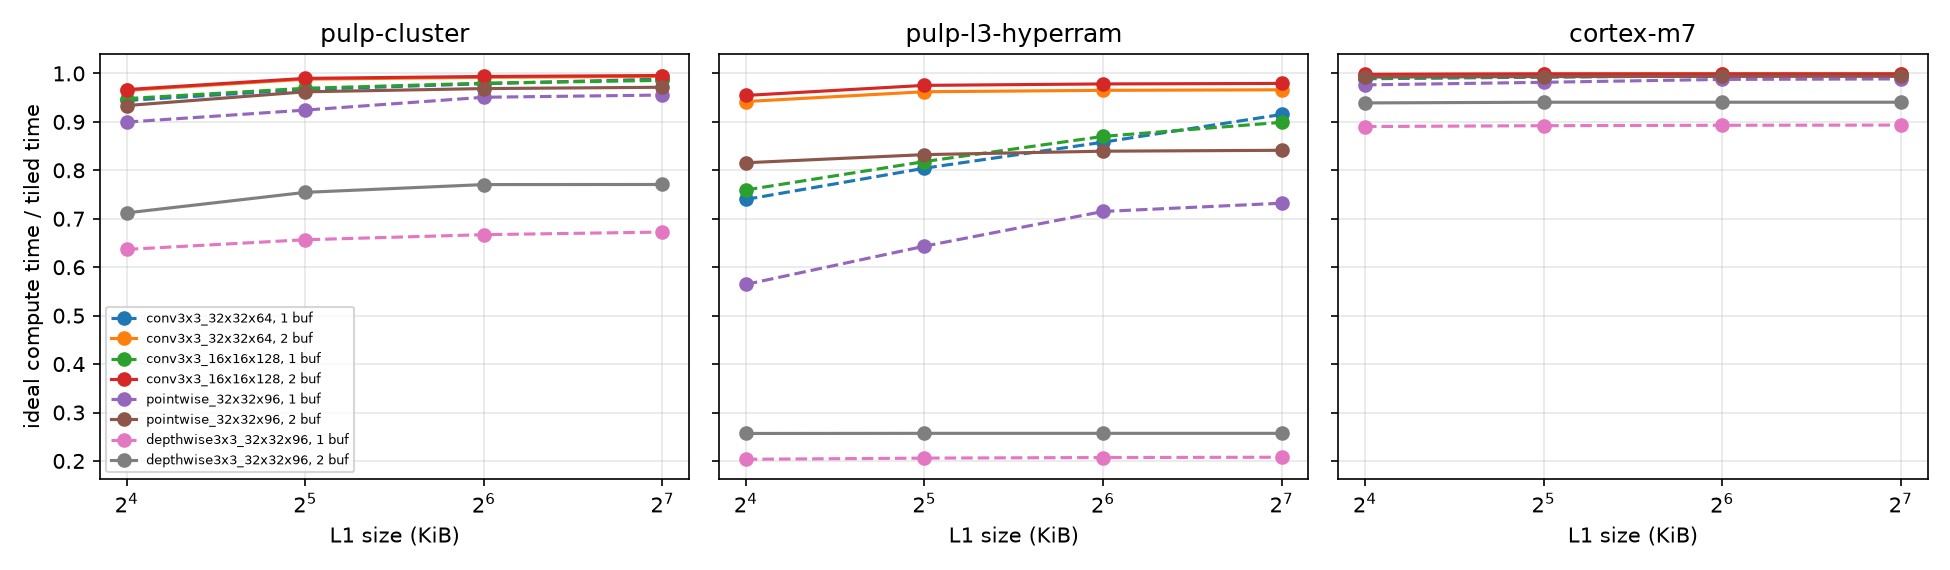
\includegraphics[width=\linewidth]{dory_efficiency.png}
\caption{本机运行的搜索结果（\texttt{dory\_efficiency.png}）。三列是三个目标，横轴 L1（16--128 KiB，对数），纵轴效率 = 理想计算周期 / 分块后总周期；
实线为双缓冲最优 tile，虚线为单缓冲最优 tile，颜色区分四种层。}\label{fig:dory}
\end{figure}

\Cref{fig:dory} 一眼能读出三件事。左列 pulp-cluster：三种普通卷积的实线都在 0.93 以上，与虚线贴得很近，双缓冲收益很小；
只有灰色的 depthwise 实线停在 0.71--0.77，粉色虚线 0.64--0.67。中列 HyperRAM：3×3 卷积的实线仍在 0.94 以上，但虚线掉到 0.74--0.92，
两线之间的空隙就是双缓冲的收益（最大 27\%）；depthwise 两条线压在 0.2--0.26 的谷底、几乎水平，L1 再大也拉不上去。
右列 Cortex-M7：除 depthwise 外所有线都挤在 0.98--1.0，虚实几乎重合——只有 2 MAC/cycle，任何层都是计算受限。

\begin{table}[H]
\centering\small
\caption{双缓冲最优 tile 的效率与双缓冲收益（L1 = 16--128 KiB 的范围，\texttt{summary.json}）}\label{tab:doryrange}
\begin{tabular}{llll}
\toprule
层 & pulp-cluster & pulp-l3-hyperram & cortex-m7 \\
\midrule
conv3x3 32×32×64 & 0.965--0.994，1.006--1.022 & 0.942--0.966，1.056--1.273 & 0.998--0.999，1.002--1.009 \\
conv3x3 16×16×128 & 0.967--0.996，1.010--1.021 & 0.955--0.979，1.089--1.257 & 0.998--0.999，1.003--1.008 \\
pointwise 32×32×96 & 0.934--0.971，1.017--1.041 & 0.816--0.841，1.149--1.445 & 0.992--0.994，1.005--1.017 \\
depthwise 32×32×96 & 0.712--0.771，1.118--1.155 & \textbf{0.257}，1.237--1.262 & 0.939--0.941，1.053--1.055 \\
\bottomrule
\end{tabular}
\end{table}

\subsection{L1 = 64 KiB 时选出的 tile}

\begin{table}[H]
\centering\small
\caption{L1 = 64 KiB、双缓冲时的最优 tile（\texttt{dory\_tiles.csv}，周期）}\label{tab:tiles64}
\begin{tabular}{llrrrrrrlrr}
\toprule
层 & 目标 & $t_h$ & $t_k$ & $t_c$ & 块数 & $m$ & $c$ & 受限 & 效率 & 收益 \\
\midrule
conv3x3 32×32×64 & cluster & 8 & 32 & 16 & 32 & 1286 & 74028 & 计算 & 0.992 & 1.013 \\
 & hyperram & 8 & 32 & 16 & 32 & 10148 & 74028 & 计算 & 0.965 & 1.125 \\
 & m7 & 8 & 32 & 16 & 32 & 2532 & 589924 & 计算 & 0.999 & 1.004 \\
\midrule
conv3x3 16×16×128 & cluster & 16 & 32 & 16 & 32 & 1254 & 74028 & 计算 & 0.994 & 1.014 \\
 & hyperram & 16 & 32 & 16 & 32 & 9892 & 74028 & 计算 & 0.978 & 1.125 \\
 & m7 & 16 & 32 & 16 & 32 & 2468 & 589924 & 计算 & 0.999 & 1.004 \\
\midrule
pointwise 32×32×96 & cluster & 2 & 96 & 96 & 16 & 1950 & 37164 & 计算 & 0.969 & 1.019 \\
 & hyperram & 4 & 96 & 32 & 24 & 7268 & 24876 & 计算 & 0.839 & 1.174 \\
 & m7 & 4 & 96 & 32 & 24 & 1812 & 196708 & 计算 & 0.994 & 1.006 \\
\midrule
depthwise 32×32×96 & cluster & 32 & 12 & 12 & 8 & 1777.5 & 7212 & 计算 & 0.771 & 1.155 \\
 & hyperram & 32 & 4 & 4 & 24 & 4760 & 2604 & \textbf{DMA} & \textbf{0.257} & 1.241 \\
 & m7 & 32 & 6 & 6 & 16 & 1767.5 & 27748 & 计算 & 0.941 & 1.053 \\
\bottomrule
\end{tabular}
\end{table}

\Cref{tab:tiles64} 是 \cref{tab:ratio} 的逐 tile 版本。3×3 卷积在 PULP + L2 上每块 $c/m\approx58$，即使换成 HyperRAM（$c/m\approx7.3$）也还是计算受限；
12 个组合里只有 depthwise + HyperRAM 一个是 DMA 受限。这与“3×3 卷积几乎总是计算受限、depthwise 和逐元素算子在片外存储上是搬运受限”的经验一致。

\subsection{depthwise + HyperRAM：效率 0.257 从哪来}

笔记里的白板估算可以直接复现这个数：depthwise 3×3、32×32×96、int8，$\text{MACs}=32\cdot32\cdot96\cdot9=884{,}736$，16 MAC/cycle 下计算 55,296 周期；
要搬的字节是输入 $34\cdot34\cdot96$ 加输出 $32\cdot32\cdot96$，共 209,280 B，1 B/cycle 下 209,280 周期。
计算只占搬运的 26\%，所以无论怎么切、开几块缓冲，效率都不会超过约 0.26；搜索结果 0.257 只比这个上界低一点（多出来的是每块 100 周期的 DMA 启动和最后一块的排空）。

从 \cref{eq:dory} 看双缓冲收益的上界：设整层 DMA 一侧（搬入 + 写回）总时间为 $D$、计算总时间为 $C$，单缓冲约 $D + C$，双缓冲约 $D + c$（只剩最后一块的计算露在外面），
比值约 $1 + C/D\approx1 + 55{,}296/209{,}280\approx1.26$。搜索得到 1.237--1.262，正好贴着这个上界。这就是摘要里“封顶于 $(m+c)/m\approx1.25$”的含义：
把写回算进 DMA 一侧，每 tile 的 DMA 约为计算的 4 倍，双缓冲只能藏住那 $1/4$。

L1 从 32 KiB 增到 128 KiB 时，depthwise + HyperRAM 的双缓冲最优 tile 一直是 $(32, 4, 4)$、24 块、17,512 B，效率一直是 0.25701：
DMA 受限时，tile 再大也不减少总字节，只是让流水的填充-排空项变大，搜索就不用多出来的 L1。

\subsection{L1 大小与双缓冲的 L1 代价}

L1 变大时 tile 数变少、每次调用开销摊薄，效率上升，但双缓冲的额外收益下降。以 \texttt{conv3x3\_32x32x64} 在 pulp-cluster 上为例：

\begin{table}[H]
\centering\small
\caption{\texttt{conv3x3\_32x32x64} @ pulp-cluster，单 / 双缓冲各自的最优 tile}\label{tab:l1sweep}
\begin{tabular}{rlrrlrrr}
\toprule
L1 KiB & 单缓冲 tile & 块数 & 效率 & 双缓冲 tile & 块数 & 效率 & 收益 \\
\midrule
16 & (4, 16, 16) & 128 & 0.944 & (4, 16, 8) & 256 & 0.965 & 1.022 \\
32 & (8, 16, 32) & 32 & 0.967 & (8, 16, 16) & 64 & 0.988 & 1.022 \\
64 & (8, 32, 64) & 8 & 0.979 & (8, 32, 16) & 32 & 0.992 & 1.013 \\
128 & (16, 64, 64) & 2 & 0.988 & (16, 32, 32) & 8 & 0.994 & 1.006 \\
\bottomrule
\end{tabular}
\end{table}

每一档 L1 上，双缓冲选出的 tile 都比单缓冲小（$t_c$ 减半或 $t_k$ 减半）、块数多 2--4 倍：这就是“输入和权重缓冲各两份”的代价。
它在这里仍然赚：双缓冲藏住的搬运（每块 1286 周期量级）比多出来的调用开销（每块 300 周期）多。效率从 0.965（16 KiB、256 块）升到 0.994（128 KiB、8 块），
与笔记中“最优点在 L1 约束边界附近，但不一定贴边”的推导一致：总时间 $\approx \text{MACs}/P + N s_{\text{call}} + \text{MACs}/(NP)$，
$N s_{\text{call}}$ 随块数 $N$ 增长、排空项随 $N$ 减小，L1 给 $N$ 一个下界。

HyperRAM 上同一层单缓冲效率只有 0.740--0.915，双缓冲 0.942--0.966；收益从 16 KiB 时的 1.273 降到 128 KiB 时的 1.056——L1 越小、tile 越碎，
每块的 DMA 启动（100 周期）越多，越需要把搬运藏起来。

\begin{findingbox}[：双缓冲是给“搬运与计算同量级”的层准备的]
12 个（层，目标）组合里，计算受限的 11 个双缓冲只多 0.2\%--45\%，其中 3×3 卷积在片上 L2 供数时只多 0.6\%--2.2\%；
唯一 DMA 受限的 depthwise + HyperRAM 收益 1.24 倍，并且被 $1 + C/D\approx1.25$ 封顶，效率仍只有 0.257。
双缓冲收益最大的是 pointwise + HyperRAM、16 KiB L1（1.445 倍）：那里 $m$ 与 $c$ 最接近（6244 对 6444 周期）。
DMA 受限时该做的是减少字节（int8 / int4 激活、depthwise 与前后 pointwise 融合、跨层分块），而不是加缓冲。
\end{findingbox}

pointwise + HyperRAM 的效率只有 0.816--0.841，主要损失在 \cref{eq:dory} 的写回项：模型里输出写回不与计算重叠，
1×1 卷积每 MAC 对应的输出字节比 3×3 多 9 倍。如果真实 DMA 能把写回也放进流水（独立的输出通道），这一行会显著变好——又回到 E16 “数引擎”的问题。

\section{本机两线程实测}\label{sec:host}

\begin{figure}[H]
\centering
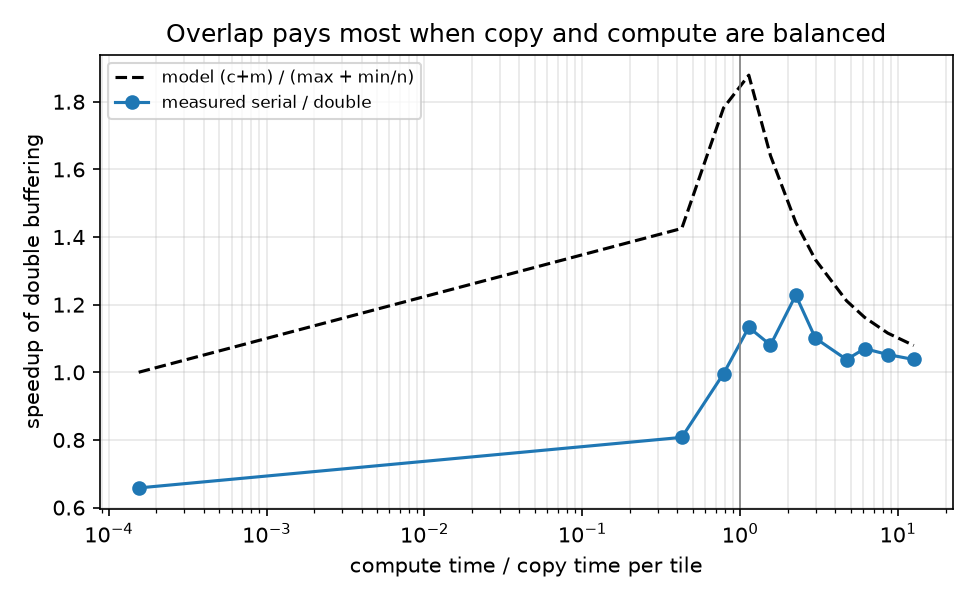
\includegraphics[width=0.85\linewidth]{dma_overlap.png}
\caption{本地 Ice Lake VM，64 KiB tile、512 块（\texttt{dma\_overlap.png}）。横轴：每 tile 计算时间 / 拷贝时间（对数）；纵轴：串行 / 双缓冲；
虚线为模型 $(c+m)/(\max+\min/n)$，实线为实测，竖线标 $c/m=1$。}\label{fig:overlap}
\end{figure}

\Cref{fig:overlap} 的虚线在 $c/m\approx1.13$ 处到峰 1.88，向两侧下降，形状就是 \cref{eq:speedup}；最左端 $c/m\approx10^{-4}$（\texttt{work}=0，只剩同步）模型为 1。
图中 $10^{-4}$ 到 0.43 之间只有两个采样点，两段直线是绘图插值，不是测量。实测曲线整体在虚线下方：
最左端只有 0.66（只做同步就慢了 34\%），在 $c/m=0.78$ 才回到 1.00，峰值 1.23 出现在 $c/m=2.25$，比模型的峰向右偏；$c/m>4$ 后两条线一起趋近 1。

\begin{table}[H]
\centering\small
\caption{本机，64 KiB tile、512 块（\texttt{dma\_measured.csv}；单 tile 时间由 CSV 除以块数得到）}\label{tab:localsweep}
\begin{tabular}{rrrrrrrr}
\toprule
\texttt{work} & $m$ ($\mu$s) & $c$ ($\mu$s) & $c/m$ & 模型加速 & 实测加速 & 实测串行 / 模型 & 实测双缓冲 / 模型 \\
\midrule
0 & 5.04 & 0.00 & 0.0002 & 1.00 & 0.66 & 0.98 & 1.48 \\
1 & 5.06 & 2.16 & 0.43 & 1.43 & 0.81 & 0.99 & 1.75 \\
2 & 5.53 & 4.34 & 0.78 & 1.78 & 1.00 & 0.97 & 1.74 \\
3 & 5.09 & 5.77 & 1.13 & 1.88 & 1.13 & 1.07 & 1.78 \\
4 & 5.03 & 7.83 & 1.56 & 1.64 & 1.08 & 1.03 & 1.56 \\
6 & 5.51 & 12.40 & 2.25 & 1.44 & 1.23 & 1.14 & 1.34 \\
8 & 5.06 & 15.15 & 3.00 & 1.33 & 1.10 & 1.05 & 1.28 \\
12 & 4.83 & 22.78 & 4.72 & 1.21 & 1.04 & 1.07 & 1.25 \\
16 & 5.08 & 31.21 & 6.14 & 1.16 & 1.07 & 1.06 & 1.15 \\
24 & 5.60 & 48.22 & 8.61 & 1.12 & 1.05 & 1.02 & 1.08 \\
32 & 4.77 & 60.00 & 12.57 & 1.08 & 1.04 & 1.07 & 1.11 \\
\bottomrule
\end{tabular}
\end{table}

\Cref{tab:localsweep} 最后两列是本报告从 CSV 多算的一步，也是理解差距的关键：\emph{串行}实测在模型的 0.97--1.14 倍以内，
\emph{双缓冲}实测却是模型的 1.08--1.78 倍。也就是说，单独测的 $m$ 和 $c$ 加起来能很好地预测串行时间，模型本身的“分段时间”没有错；
错的是 \cref{eq:t2} 背后的假设——两段可以同时进行而互不拖慢。以 \texttt{work}=3 为例，双缓冲每块 10.28~$\mu$s，模型 5.78~$\mu$s，
多出的 4.5~$\mu$s 几乎等于一次拷贝（5.09~$\mu$s）：重叠之后拷贝像是没被藏住。

\subsection{固定 $c/m$、改 tile 大小}

\begin{table}[H]
\centering\small
\caption{本机，\texttt{work}=4，改 tile 大小（\texttt{dma\_measured.csv}，时间单位 $\mu$s）}\label{tab:localtiles}
\begin{tabular}{rrrrrrrr}
\toprule
tile & 块数 & $m$ ($\mu$s) & $c/m$ & 模型加速 & 实测加速 & 双缓冲每块 实测 / 模型 & 每块多出 \\
\midrule
4 KiB & 4096 & 0.30 & 1.15 & 1.87 & 0.61 & 1.18 / 0.34 & 0.84 \\
16 KiB & 1024 & 1.20 & 1.24 & 1.81 & 0.71 & 3.97 / 1.48 & 2.49 \\
64 KiB & 256 & 5.01 & 1.54 & 1.65 & 0.96 & 13.87 / 7.71 & 6.15 \\
256 KiB & 64 & 21.01 & 1.50 & 1.65 & 1.02 & 52.65 / 31.91 & 20.74 \\
1 MiB & 16 & 110.98 & 2.28 & 1.40 & 1.08 & 324.37 / 260.47 & 63.90 \\
\bottomrule
\end{tabular}
\end{table}

4 KiB 时双缓冲每块 1.18~$\mu$s，模型只有 0.34~$\mu$s，多出约 0.8~$\mu$s，比搬运本身（0.30~$\mu$s）还长，于是双缓冲比串行慢 39\%；tile 增大到 1 MiB 时实测回到 1.08 倍。
注意“每块多出”这一列并不是常数：它从 0.84~$\mu$s 涨到 63.9~$\mu$s，随 tile 字节增长，但每 KiB 的份额从 0.21~$\mu$s 降到 0.06~$\mu$s。
这说明损失有两部分：一部分与块数成正比（每块一次跨线程握手：一次 release-store 加一次对方的 acquire 自旋，缓存行在两个核之间来回）；
另一部分与字节成正比（两个线程共享 L2/L3 与 DRAM 带宽、拷贝本身占用核心的 load/store 端口；计算线程读的 tile 是另一个核刚写的，
cache line 要从拷贝核迁移过来）。前者让 tile 不能太小，后者让 tile 再大也拿不到模型的加速比。这两部分的拆分是由这一列的形状推出的，没有用计数器确认。

\begin{findingbox}[：在 CPU 上，固定开销与资源共享吃掉了重叠收益]
本机两线程实测双缓冲 0.61--1.23 倍，模型 1.00--1.88 倍。串行时间被模型准确预测（0.96--1.14 倍），双缓冲时间是模型的 1.08--3.48 倍，
所以损失全在“重叠”本身。MCU 的 DMA 引擎有独立的总线端口、不抢计算核的 load/store 端口，更接近模型；
但每次 DMA 的启动开销（\cref{tab:targets} 里假设 20--100 周期）同样让 tile 不能太小——这一点 CPU 上的 4 KiB 点和 MCU 模型是一致的。
\end{findingbox}

\section{本机与服务器对照}\label{sec:cross}

同一份 \texttt{dma.cpp} 与 \texttt{run\_experiments.py} 在 Xeon 8470Q 上完整重跑了 model、dory、measure 三步，结果在
\nolinkurl{artifacts/raw/xeon8470q/} 与 \nolinkurl{artifacts/figures/xeon8470q/}。

\subsection{模型部分：逐位复现}

\begin{figure}[H]
\centering
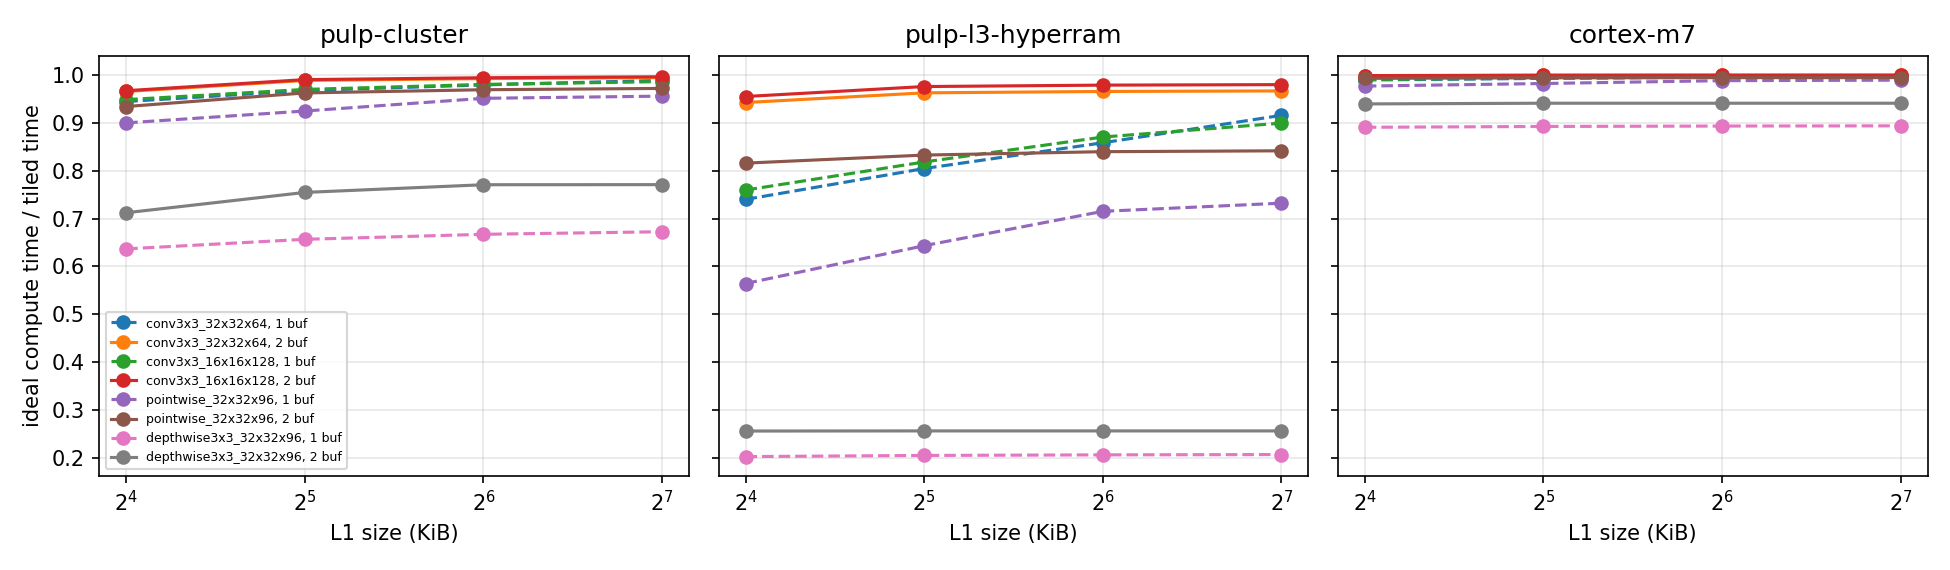
\includegraphics[width=\linewidth]{xeon8470q/dory_efficiency.png}
\caption{服务器上重跑的 Dory 式搜索（\texttt{xeon8470q/dory\_efficiency.png}）。轴与图例同 \cref{fig:dory}。}\label{fig:dory-srv}
\end{figure}

\Cref{fig:dory-srv} 与 \cref{fig:dory} 肉眼无法区分：两个 \texttt{summary.json} 中 96 个 \texttt{dory:*} 键逐位相同。
这一步是纯 Python 的确定性计算，复现它的意义只是确认“服务器上跑的是同一份代码”——后面实测曲线的差异不能归咎于代码或参数漂移。

\subsection{实测部分：模型预测加速，服务器全部变慢}

\begin{figure}[H]
\centering
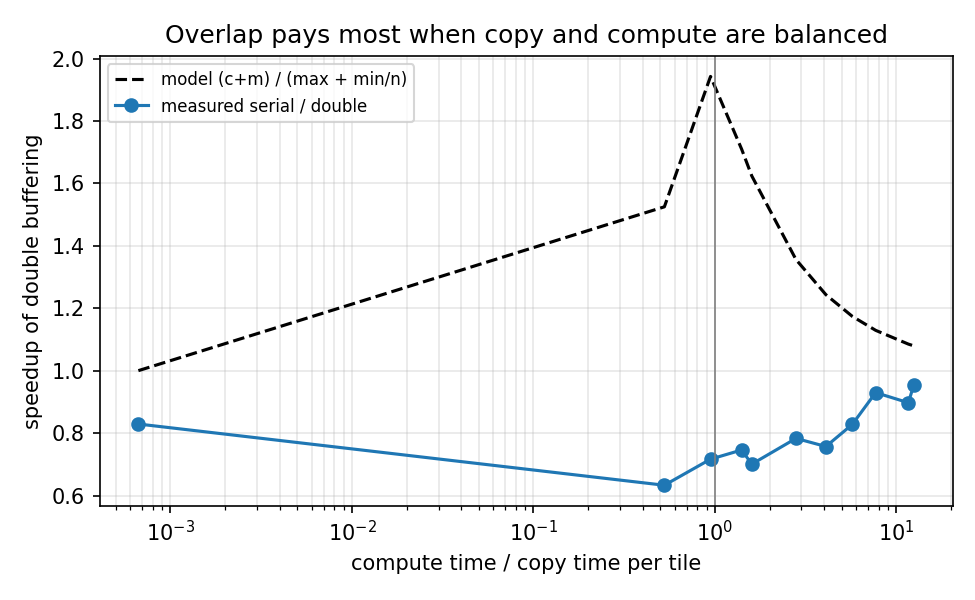
\includegraphics[width=0.85\linewidth]{xeon8470q/dma_overlap.png}
\caption{服务器，64 KiB tile、512 块（\texttt{xeon8470q/dma\_overlap.png}）。轴同 \cref{fig:overlap}。}\label{fig:overlap-srv}
\end{figure}

\Cref{fig:overlap-srv} 的模型曲线与本机几乎相同，在 $c/m=0.95$ 处到峰 1.94（服务器上测得的 $m$ 与 $c$ 恰好更接近相等）。
实测曲线却整条在 1 以下：从 $c/m=0.53$ 处的 0.63 开始，在 $c/m=1$ 附近只有 0.72，随后缓慢爬升到 $c/m\approx12$ 时的 0.95，没有峰。
与本机相反，服务器上 \texttt{work}=0（只做同步）的 0.83 反而比 \texttt{work}=1 的 0.63 好：一旦计算线程真的去读 tile，损失就变大。

\begin{figure}[H]
\centering
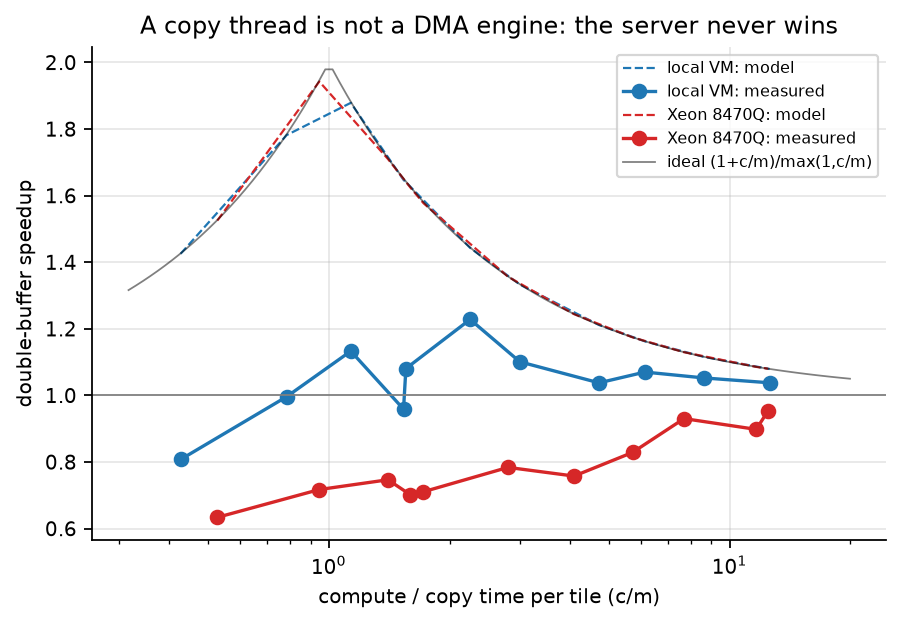
\includegraphics[width=0.85\linewidth]{xeon8470q/model_vs_measured.png}
\caption{模型预测与两台主机的实测放在同一张图（\texttt{xeon8470q/model\_vs\_measured.png}）。蓝：本地 VM；红：Xeon 8470Q；
虚线为各自用测得的 $m$、$c$ 代入的模型；灰线为 $n\to\infty$ 的理想上界 $(1+c/m)/\max(1,c/m)$；横线标 1。}\label{fig:mvm}
\end{figure}

\Cref{fig:mvm} 是本报告最重要的一张图。三条模型线（蓝虚、红虚、灰实）几乎重合，峰都在 $c/m\approx1$：拷贝与计算等长时双缓冲收益最大。
本地实测（蓝实线）的峰也大致在这里，只是被压低到 1.13--1.23；服务器实测（红实线）整体平移到 1 以下，峰的位置消失了。
这个\emph{形状}差异说明问题：如果损失来自“重叠得不够”，实测曲线应与模型同形、只是更矮；服务器曲线没有峰，说明第二个线程本身带来了与 $c/m$ 关系不大的固定成本。
图中蓝线在 $c/m\approx1.55$ 处有一个竖直的折线（0.96 与 1.08 两点），是因为这张图同时画了扫描一（512 块，1.08）和扫描二中 64 KiB、256 块那一行（0.96），见 \cref{sec:caveat}。

\begin{table}[H]
\centering\small
\caption{64 KiB tile、512 块，两台主机（\texttt{dma\_measured.csv} 与 \texttt{xeon8470q/dma\_measured.csv}）}\label{tab:cross}
\begin{tabular}{rrrrrrr}
\toprule
 & \multicolumn{3}{c}{本地 VM} & \multicolumn{3}{c}{Xeon 8470Q} \\
\cmidrule(lr){2-4}\cmidrule(lr){5-7}
\texttt{work} & $c/m$ & 模型 & 实测 & $c/m$ & 模型 & 实测 \\
\midrule
0 & 0.0002 & 1.00 & 0.66 & 0.0007 & 1.00 & 0.83 \\
1 & 0.43 & 1.43 & 0.81 & 0.53 & 1.53 & 0.63 \\
2 & 0.78 & 1.78 & 1.00 & 0.95 & 1.94 & 0.72 \\
3 & 1.13 & 1.88 & 1.13 & 1.40 & 1.71 & 0.75 \\
4 & 1.56 & 1.64 & 1.08 & 1.60 & 1.62 & 0.70 \\
6 & 2.25 & 1.44 & 1.23 & 2.80 & 1.36 & 0.78 \\
8 & 3.00 & 1.33 & 1.10 & 4.09 & 1.24 & 0.76 \\
12 & 4.72 & 1.21 & 1.04 & 5.72 & 1.17 & 0.83 \\
16 & 6.14 & 1.16 & 1.07 & 7.69 & 1.13 & 0.93 \\
24 & 8.61 & 1.12 & 1.05 & 11.64 & 1.09 & 0.90 \\
32 & 12.57 & 1.08 & 1.04 & 12.47 & 1.08 & 0.95 \\
\bottomrule
\end{tabular}
\end{table}

\begin{table}[H]
\centering\small
\caption{服务器，\texttt{work}=4，改 tile 大小（\texttt{xeon8470q/dma\_measured.csv}，时间单位 $\mu$s）}\label{tab:srvtiles}
\begin{tabular}{rrrrrrrr}
\toprule
tile & 块数 & $m$ ($\mu$s) & $c/m$ & 模型加速 & 实测加速 & 双缓冲每块 实测 / 模型 & 每块多出 \\
\midrule
4 KiB & 4096 & 0.17 & 1.23 & 1.82 & 0.44 & 0.81 / 0.21 & 0.60 \\
16 KiB & 1024 & 0.66 & 1.14 & 1.87 & 0.62 & 2.52 / 0.75 & 1.77 \\
64 KiB & 256 & 3.10 & 1.72 & 1.58 & 0.71 & 11.17 / 5.35 & 5.82 \\
256 KiB & 64 & 13.30 & 1.73 & 1.56 & 0.89 & 38.88 / 23.19 & 15.69 \\
1 MiB & 16 & 74.20 & 2.01 & 1.45 & 0.85 & 214.67 / 153.88 & 60.79 \\
\bottomrule
\end{tabular}
\end{table}

把两张表并排读：
\begin{itemize}
  \item \textbf{服务器的拷贝更快，于是固定成本占比更大。} 64 KiB 拷贝本机约 5.0~$\mu$s（约 13 GB/s），服务器约 2.7--3.4~$\mu$s（19--25 GB/s）；
        但双缓冲每块多出的时间服务器是 3.8--6.7~$\mu$s，本机是 2.4--6.8~$\mu$s，量级相同。多出的时间已经超过服务器上一次拷贝本身，所以双缓冲必然慢于串行。
  \item \textbf{串行依旧准。} 服务器上串行实测是模型的 0.81--1.11 倍，双缓冲是模型的 1.16--3.91 倍（\texttt{work}=0 时为 0.99）。与本机一样，损失全部在重叠路径。
  \item \textbf{tile 扫描同形。} 两台机器上“每块多出”都随 tile 增大（服务器 0.60 $\to$ 60.8~$\mu$s），实测加速都在 4 KiB 时最差（本机 0.61、服务器 0.44）。
        服务器上最好的一点也只有 256 KiB 时的 0.89。
\end{itemize}

服务器比本机多两个干扰源：两个线程可能落在 mesh 上相距较远的核上，跨核交接 tile 时每条 cache line 都要经过 mesh 搬一次；
cgroup 只给 22 个 CPU 的配额、宿主上还有其他租户。前者由 Sapphire Rapids 的 mesh 结构与“多出时间随字节增长”的形状推出，后者来自 edge-runtime-server 报告的环境记录；
两者都没有用计数器或绑核对照实验拆开。

\begin{findingbox}[：拷贝线程不是 DMA 引擎]
双缓冲模型假设“拷贝”与“计算”使用互不干扰的资源。在 CPU 上二者都是 load/store、共享 L2/L3 与内存控制器，tile 还要在两个核之间迁移，
本机还能在 $c/m\approx1$--2 拿到 1.13--1.23 倍，服务器上 11 个点全部低于 1（0.63--0.95）。模型只在拷贝由独立硬件完成时成立：
MCU 的 DMA 控制器、GPU 的 copy engine / TMA。这是面试里“为什么在 CPU 上做软件流水不一定有收益”的实测证据。
\end{findingbox}

\section{面试追问}\label{sec:iq}

\begin{iqbox}{开了双缓冲，延迟能减半吗？}
只有 $m\approx c$ 且块数多时才接近。E15：$T_2 = n\max(m,c)+\min(m,c)$，加速比 $(m+c)/(\max+\min/n)$，上界 $1+\min/\max\le2$，省下的是较短的那一侧乘 $n-1$。
本仓库模型里 $c/m=1$、64 块是 65 对 128；$c/m=0.125$ 只快 12\%。Dory 式搜索里 3×3 卷积在片上 L2 供数时只多 0.6\%--2.2\%，
depthwise 从 HyperRAM 供数是 DMA 受限，1.24 倍、被 1.25 封顶。

\emph{常见错答}：“双缓冲把搬运完全藏住，所以总时间等于计算时间”——只有计算受限时才对，DMA 受限时总时间等于搬运时间，多一块缓冲造不出带宽。
\end{iqbox}

\begin{iqbox}{只有一个 DMA 通道，搬入、计算、搬出做三级流水还有用吗？}
没用。E16 的 $\sum s_i + (n-1)\max s_i$ 要求每级一个独立引擎。搬入、搬出共用一个通道时，两者在同一个引擎上串行，DMA 一侧每块是 $m_{\text{in}}+m_{\text{out}}$，
退化成两级。模拟里 $m=1$、$o=0.5$、$c\le1$、64 块时，独立通道约 65，共享通道 96 $=64\times1.5$，计算完全被藏住，瓶颈是通道本身。
所以先数引擎，再定缓冲数；本模型里写回不与计算重叠，pointwise + HyperRAM 的效率只有 0.82--0.84，主要就损失在这里。
\end{iqbox}

\begin{iqbox}{双缓冲的代价是什么？最优 tile 为什么不是最小，也不是最大？}
代价是 L1：输入和权重缓冲各两份（E17），原本放得下的 tile 放不下，tile 变小、块数变多，每块付一次 DMA 启动和一次内核调用开销（E18）。
\texttt{conv3x3\_32x32x64} 在 pulp-cluster 上每档 L1 双缓冲选出的 tile 都比单缓冲小，块数多 2--4 倍（16 KiB 时 256 对 128 块）。
tile 太小，$N s_{\text{call}}$ 与 DMA 启动占比上升；tile 太大，放不进 L1，或者流水的填充-排空项 $\min(m,c)$ 变大。
所以效率随 L1 从 0.965 升到 0.994，但双缓冲的额外收益从 1.022 降到 1.006。不计开销项时，搜索会选出最小 tile——这是本仓库早期版本犯过的错。
\end{iqbox}

\begin{iqbox}{在 CPU 上用一个线程做 memcpy、另一个线程计算，为什么反而更慢？CPU 上该怎么做？}
双缓冲的前提是搬运由独立硬件完成，不占计算单元的发射槽、不污染计算单元的缓存。CPU 上拷贝线程与计算线程争用同一套 load/store 端口与缓存层次，
还要付每块一次的跨线程握手和 cache line 跨核迁移。本机实测 0.61--1.23 倍（4 KiB 时每块多出约 0.8~$\mu$s，比搬运本身还长），
服务器上 0.63--0.95 倍、没有一个点超过 1。一个可检查的事实：两台机器上串行时间都被 $n(m+c)$ 准确预测，双缓冲时间却是模型的 1.1--3.9 倍。
CPU 上等价的做法是硬件预取或软件 \texttt{prefetch} 指令，让同一个核在计算时把下一块拉进缓存，而不是另起一个拷贝线程。
\end{iqbox}

\begin{iqbox}{怎么判断一层是 DMA 受限？受限之后还能做什么？}
算每个 tile 的 $\text{MACs}/P$ 与 $\text{bytes}/\text{BW}$，前者小就是 DMA 受限。量级上，3×3 卷积的比值约 $9t_k\,\text{BW}/P$，depthwise 约 $9\,\text{BW}/P$：
PULP + L2 时 depthwise 约 4.5（计算受限，效率 0.77），换成 HyperRAM 约 0.56（DMA 受限，效率 0.257）。在板上也可以把计算换成空循环，看总时间变不变。
DMA 受限时加缓冲没用，要减少字节：int8 甚至 int4 激活；把 depthwise 与前后的 pointwise 融合，让中间激活不出 L1；或者跨层分块、提前把输入放进 L2。
\end{iqbox}

\section{结论}\label{sec:conclusion}

\begin{findingbox}[：模型]
事件模拟与闭式逐点相等：单缓冲 $n(m+c)$，双缓冲 $n\max(m,c)+\min(m,c)$，加速比只取决于 $c/m$ 与块数，上界 $1+\min/\max\le2$。
搬入、搬出共用一个 DMA 通道时，三级流水退化成两级（$c/m\le1$ 时 96 对 65）。
\end{findingbox}

\begin{findingbox}[：搜索]
在假设的三个目标、四档 L1 上，3×3 卷积全部计算受限，双缓冲只多 0.2\%--27\%（片上 L2 供数 0.6\%--2.2\%，HyperRAM 供数 5.6\%--27\%）；
depthwise 从 HyperRAM 供数是唯一的 DMA 受限组合，效率 0.257，双缓冲 1.24--1.26 倍，被 $1 + C/D\approx1.25$ 封顶。
双缓冲让 tile 变小、块数变多，但在这些层上这笔账仍然赚。
\end{findingbox}

\begin{findingbox}[：实测]
本机两线程双缓冲 0.61--1.23 倍（模型 1.00--1.88 倍），服务器 64 KiB tile 的 11 个点全部 0.63--0.95 倍。两台机器上串行时间都被模型准确预测，
双缓冲时间是模型的 1.1--3.9 倍：模型的分段时间对，“拷贝与计算互不干扰”的假设在 CPU 上不成立。拷贝线程不是 DMA 引擎。
\end{findingbox}

\section{20 秒讲法}\label{sec:pitch}

双缓冲把总时间从 $n(m+c)$ 降到 $n\max(m,c)+\min(m,c)$，省下的永远是较短的那一侧，所以只有搬运和计算差不多长时才接近 2 倍。
我在 Dory 式 tile 搜索里看到，3×3 卷积在 MCU 上几乎都是计算受限，双缓冲只多百分之几；depthwise 从片外 HyperRAM 供数是搬运受限，
效率只有 0.257，双缓冲 1.24 倍就封顶了，这时该减字节而不是加缓冲。我又在 CPU 上用拷贝线程模拟 DMA：串行时间模型算得很准，
双缓冲却在服务器上全部变慢，因为拷贝和计算抢同一套缓存和端口——模型只在搬运有独立硬件时成立。

\section{不能推出的结论}\label{sec:caveat}

\begin{caveatbox}
\begin{itemize}
  \item 本机和服务器的“DMA”是一个 CPU 线程，与真实 DMA 引擎的行为（独立端口、描述符队列、中断）不同；本机实测只验证“固定开销与资源共享会吃掉重叠收益”这一条，
        不能推出任何 MCU / NPU 上双缓冲的实际加速比。
  \item 搜索结果的绝对周期数依赖假设的目标参数（\cref{tab:targets}）；结论只取相对关系（哪类层计算受限、双缓冲加速上界），不能当成 GAP8 或 STM32 的实测。
  \item 搜索模型只保留搬运、计算与每次调用开销三项，没有 SIMD 宽度对齐、权重常驻和跨层融合；输出写回被假设为不与计算重叠，pointwise / depthwise 在 HyperRAM 上的效率因此偏保守。
  \item “每块多出的时间分成握手与带宽共享两部分”“服务器上 cache line 跨 mesh 迁移”是由时间随 tile 大小的形状推出的，没有硬件计数器（两台机器都没有 perf 权限），
        也没有做绑核对照实验；服务器上两个线程被调度到哪两个核没有记录，cgroup 限流与其他租户的噪声不能排除。
  \item \texttt{summary.json} 的键是 \texttt{tile\{KiB\}k\_work\{w\}}，64 KiB、\texttt{work}=4 在两次扫描里各有一行（512 块与 256 块），后写入的 256 块那一行覆盖了前者。
        README 的跨主机表与 \cref{fig:mvm} 用的是 256 块那一行（本机 0.96、服务器 0.71），\cref{fig:overlap,fig:overlap-srv} 与 \cref{tab:cross} 用的是 512 块那一行（本机 1.08、服务器 0.70）。两者都是真实测量，结论不变。
  \item 每点只有 5 次重复取中位数，没有给出离散度；本机曲线在 $c/m = 1.5$--3 之间的锯齿（1.08、1.23、1.10）不应过度解读。
\end{itemize}
\end{caveatbox}

\section{复现}\label{sec:repro}

\begin{lstlisting}[language=bash]
cd solutions/edge-runtime/dma-double-buffer
python -m pytest -q tests                              # simulator == closed forms; tiles fit L1; double >= single; C++ smoke
python scripts/run_experiments.py --only model dory    # pipeline_model.csv, dory_tiles.csv, dory_efficiency.png (seconds)
python scripts/run_experiments.py --only measure       # dma_measured.{jsonl,csv}, dma_overlap.png (~10 s, idle machine)
python scripts/run_experiments.py --repeats 5          # all three steps + summary.json
\end{lstlisting}

\texttt{measure} 会用 \texttt{edge\_harness.cpp.build} 编译 \texttt{cpp/dma.cpp}（头文件在 \nolinkurl{edge_harness/include}），
依次运行 \texttt{--mode=sweep --tile-kib=64 --tiles=512} 与 \texttt{--mode=tiles --work=4}。
原始数据在 lab 的 \nolinkurl{artifacts/raw/}，服务器结果在其下的 \nolinkurl{xeon8470q/}；
\texttt{claims.json} 中 \texttt{dma-*} 五项（depthwise 效率 0.257 与 1.24 倍、conv3x3 128 KiB 效率 0.994、本机最好 1.23 倍、4 KiB 0.61 倍）对本机 \texttt{summary.json} 做数值校验。


\begin{thebibliography}{99}
\bibitem{dory} A.~Burrello, A.~Garofalo, N.~Bruschi, et al. DORY: Automatic End-to-End Deployment of Real-World DNNs on Low-Cost IoT MCUs. \emph{IEEE Transactions on Computers}, 70(8), 2021.
\bibitem{mcunet} J.~Lin, W.-M.~Chen, Y.~Lin, J.~Cohn, C.~Gan, S.~Han. MCUNet: Tiny Deep Learning on IoT Devices. \emph{NeurIPS}, 2020.
\bibitem{gpipe} Y.~Huang, Y.~Cheng, A.~Bapna, et al. GPipe: Efficient Training of Giant Neural Networks using Pipeline Parallelism. \emph{NeurIPS}, 2019.
\end{thebibliography}

\end{document}
